\documentclass[sigchi]{acmart} % authorversion=true
\usepackage{booktabs} % For formal tables

%\settopmatter{printacmref=false}

\newcommand{\RR}{I\!\!R} %real numbers
\newcommand{\Nat}{I\!\!N} %natural numbers
\newcommand{\CC}{I\!\!\!\!C} %complex numbers

\begin{document}

\copyrightyear{2017} 
\acmYear{2017} 
\setcopyright{acmlicensed}
\acmConference{AM '17}{August 23--26, 2017}{London, United Kingdom}\acmPrice{15.00}\acmDOI{10.1145/3123514.3123556}
\acmISBN{978-1-4503-5373-1/17/08}

\title{Deep Models for Ensemble Touch-Screen Improvisation}

\author{Charles P. Martin}
\orcid{0000-0001-5683-7529}
\affiliation{%
  \institution{Department of Informatics}
  \streetaddress{University of Oslo, Norway}
}
\email{charlepm@ifi.uio.no}

\author{Kai Olav Ellefsen}
\orcid{1234-5678-9012} %% todo fix this.
\affiliation{%
  \institution{Department of Informatics}
  \streetaddress{University of Oslo, Norway} 
}
\email{kaiolae@ifi.uio.no}

\author{Jim Torresen}
\orcid{1234-5678-9012} %% todo fix this.
\affiliation{%
  \institution{Department of Informatics}
  \streetaddress{University of Oslo, Norway}
}
\email{jimtoer@ifi.uio.no}

\begin{abstract}
  For many, the pursuit and enjoyment of musical performance goes hand-in-hand with collaborative creativity, whether in a choir, jazz combo, orchestra, or rock band. However, few musical interfaces use the affordances of computers to create or enhance ensemble musical experiences. One possibility for such a system would be to use an artificial neural network (ANN) to model the way other musicians respond to a single performer. Some forms of music have well-understood rules for interaction; however, this is not the case for free improvisation with new touch-screen instruments where styles of interaction may be discovered in each new performance. This paper describes an ANN model of ensemble interactions trained on a corpus of such ensemble touch-screen improvisations. The results show realistic ensemble interactions and the model has been used to implement a live-performance system where a lead performer is accompanied by the predicted and sonified touch-gestures of two virtual players.
\end{abstract}

\begin{CCSXML}
<ccs2012>
<concept>
<concept_id>10010147.10010257.10010293.10010294</concept_id>
<concept_desc>Computing methodologies~Neural networks</concept_desc>
<concept_significance>400</concept_significance>
</concept>
<concept>
<concept_id>10010405.10010469.10010475</concept_id>
<concept_desc>Applied computing~Sound and music computing</concept_desc>
<concept_significance>400</concept_significance>
</concept>
</ccs2012>
\end{CCSXML}

\ccsdesc[400]{Computing methodologies~Neural networks}
\ccsdesc[400]{Applied computing~Sound and music computing}

\keywords{deep learning, RNN, ensemble interaction, touch screen
  performance, mobile music}

\maketitle

\section{Introduction}

The proliferation of touch-screen enabled devices over the past decade
has resulted in many creative digital musical instrument designs. One
appealing aspect of these devices is that they are often portable and
suggest group performances among friends. Several researchers have
explored how these devices can be used in ensemble situations such as
Wang et al.'s \emph{MoPho} mobile phone orchestra~\cite{Wang:2014cs},
Schiemer's \emph{Pocket Gamelan} works~\cite{Greg-Schiemer:2007mz},
and Snyder's marching band of DIY mobile device powered
instruments~\cite{Snyder:2014dp}. These works demonstrate the very
wide creative space of mobile computer music with resulting
applications frequently appealing to non-expert users as
well~\cite{Wang:2014ul, Hamilton:2011aa}.

\begin{figure}
  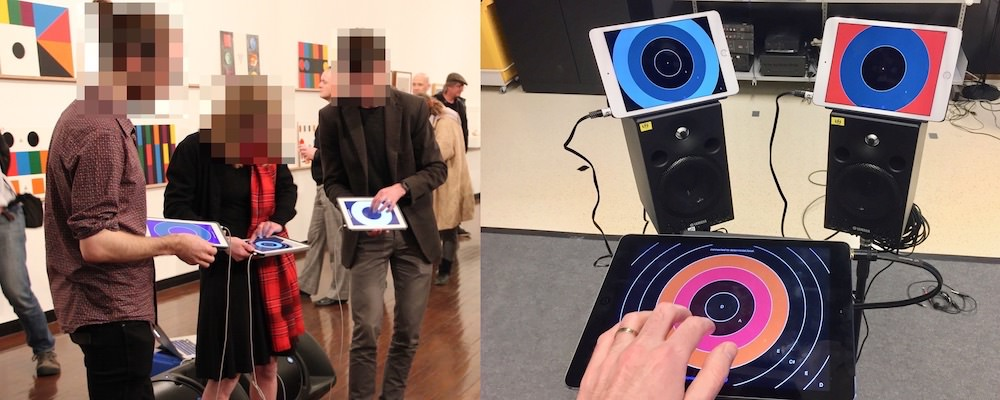
\includegraphics[width=\columnwidth]{neural-mode-ensemble}
  \caption{Data from more than 150 collaborative sessions (left) has
    been used to create a neural model of ensemble interaction
    focused on touch interaction, and a prototype system that
    accompanies a live performer
    (right).}\label{fig:performance-and-system}
\end{figure}

In previous research, Martin et al.~\cite{Martin:2016rm} captured a
data-set of more than 150 collaborative performances on mobile
instruments as part of a project exploring the design and impact of
networked mobile music interfaces (e.g., the left side of Figure
\ref{fig:performance-and-system}). This data-set included both raw
touch-data and time series of interpreted touch-gestures sampled at a
fixed interval. In the present research, we use this data-set to train
an artificial neural network (ANN), gesture-RNN, that imitates the
behaviour of the ensemble based on the input of one user. We also
present an application for the ANN in a system to automatically
accompany individual users of a mobile music app, thus extending the
experience of collaborative creativity to users and situations where a
live performance would not be possible.

Many improvised styles (e.g., jazz), have ensemble interactions based
on well-defined rules. Machine learning systems such as the
\emph{Reflexive Looper}\cite{Pachet:2013kq} and
\emph{SongSmith}~\cite{Morris:2008qe} take advantage of these rules to
create appropriate accompaniments. In the present research, the
improvised performances were ``free'', that is, performers were
allowed to perform in any way they wished within the constraints of
the touch-screen instruments. While it is clear that the performances
contained interaction between players, it is not clear how this
occurred. Thus prediction of this interaction can only be learned from
the data, without assistance from music theory.

It has previously been shown that long short-term memory (LSTM)
recurrent neural networks (RNNs) can be used for composing blues
music~\cite{Eck:2007rw}, folk tunes~\cite{Sturm:2016rz}, as well as
polyphonic music~\cite{Walder:2016le}. These networks have not, so
far, been applied to free-form improvised music using new interfaces
such as touch-screens. In this work, we demonstrate that such networks
can learn and generate these ensemble interactions. We also introduce
a real-time performance application using our ensemble interaction
RNN.

\subsection{Interpreting Touch Data}

Collaborative touch-screen interaction data was obtained from a
publicly-available corpus of collaborative touch-screen
performances~\cite{Martin:2016fc}. This corpus includes data from more
than 150 performances from rehearsals, concerts, installations, and
demonstrations. For the present research, only ensemble improvisation
data from this corpus was used. This consisted of 72 improvised
ensemble performances with a total time of 9.8 hours.

Previous work has defined a method for interpreting raw touch
information (i.e., the time and location of taps and swipes) as a
sequence of continuous touch gestures~\cite{Martin:2015jk} such as
``slow taps'', ``small swirls'', and ``fast swipes''. The resulting
sequences can be analysed to examine the structure of performances.

Working with this high-level data has advantages and disadvantages.
The state space is small (there are only 9 gestures in the vocabulary)
and these are sampled at a regular rate (1Hz) which reduces the
complexity of the data. Plots of these gesture sequences resemble
graphical scores and changes in performance style across the ensemble
can be seen at a glance. The gesture sequences, however, do not have a
one-to-one mapping with interaction in the app (e.g., tapping in any
part of the screen could be interpreted as the ``slow taps'' gesture)
so sonification of new sequences requires further processing into
appropriate touch data.

\section{ANN Model for Ensemble Performances}

Our neural network model, gesture-RNN, is designed to generate an
ensemble score of gesture sequences based on the real improvisation of
one player. Two versions of the gesture-RNN were trained corresponding
to different ensemble situations: duets and quartets. Each network
uses the same architecture of a recurrent neural network (RNN) with
long short-term memory (LSTM) cells. This architecture mirrors the
\emph{folkRNN} system described by Sturm et al.~\cite{Sturm:2016rz}
and consists of three layers of 512 LSTM cells followed by a
fully-connected softmax layer. In each case, the networks were trained
with mini-batches of 64 performance examples each consisting of 120
time-steps. Each of these examples corresponds to a 2-minute excerpt
of a real collaborative performance. The networks were implemented in
TensorFlow and were trained on an Nvidia GeForce
GTX 1080 GPU.

\subsection{Representing Ensemble Behaviour}

The gesture-RNNs were trained to output the gestural states of the
ensemble, given input of the current lead player's state and the state
of the ensemble at the previous time step. This arrangement is
illustrated in Figure \ref{fig:nn-ensemble-training}. As the training
data consisted of completely free improvisations, any player could be
taken as the lead, so several training examples could be generated from
a single slice of a performance.

\begin{figure}
  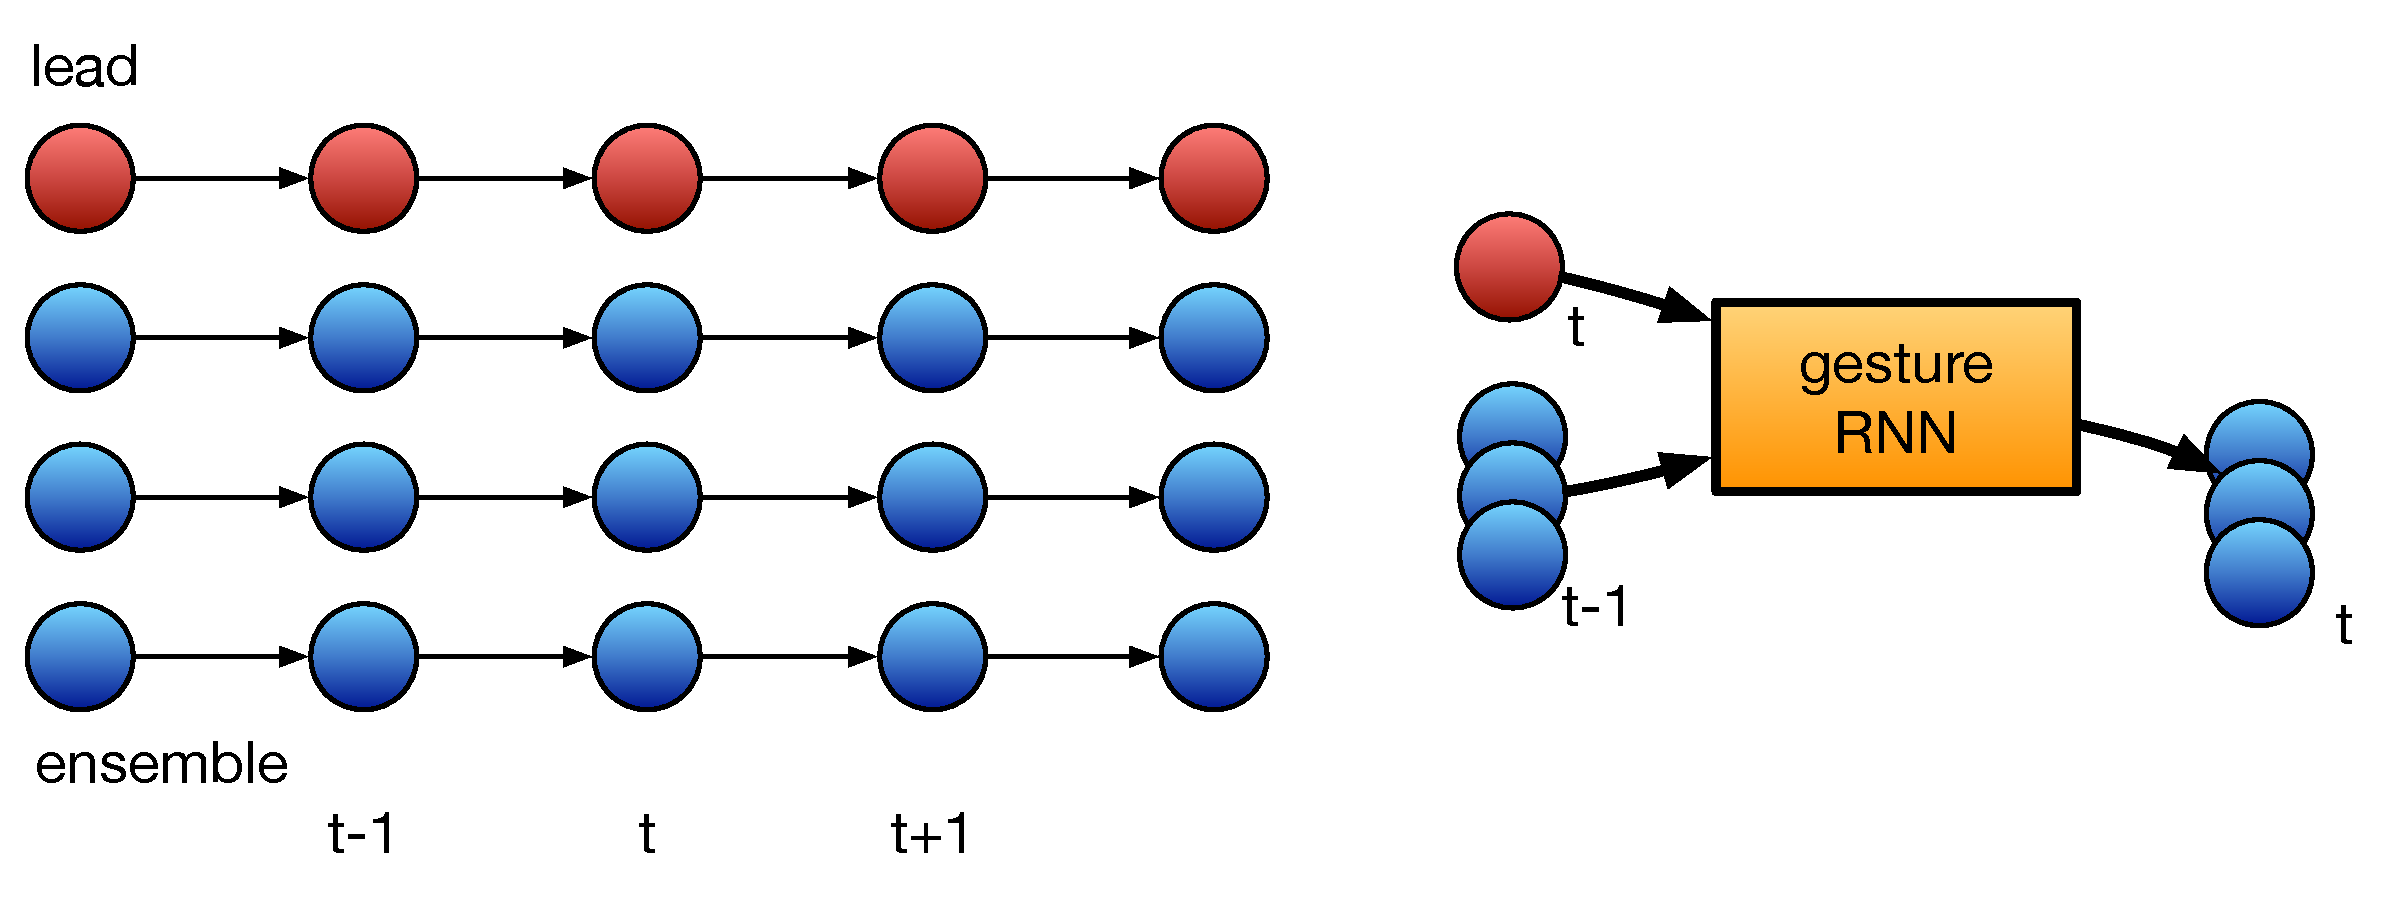
\includegraphics[width=\columnwidth]{nn-ensemble-training}
  \caption{The gesture-RNN was trained to predict the ensemble's
    gestural states given the current lead state and previous ensemble
    states.}\label{fig:nn-ensemble-training}
\end{figure}

In the data-set, each performer's actions are represented by one of
nine touch-gestures (including ``nothing''), these are stored as
integers in the interval $[0,8]$. We define a simple encoding
$\mathbb{N}_{9}^n \rightarrow \mathbb{N}_{9^n}$ to represent multiple
performers as one positive integer as follows. Given a set of
performer states $g_1, g_2, \ldots, g_n$, where the $g_i \in G$ (a
finite set of $j$ states), the states can be encoded as:
%\begin{equation}
$ g_1j^0 + g_2j^1 + g_3j^2 + \ldots + g_nj^{n-1} $.
%\end{equation}
This encoding allows any ensemble state or combination of lead player
and ensemble states to be represented as a unique integer and thus as
a one-hot encoding on the inputs and outputs of the neural network.

\subsection{Duet}

\begin{figure}
  \centering
  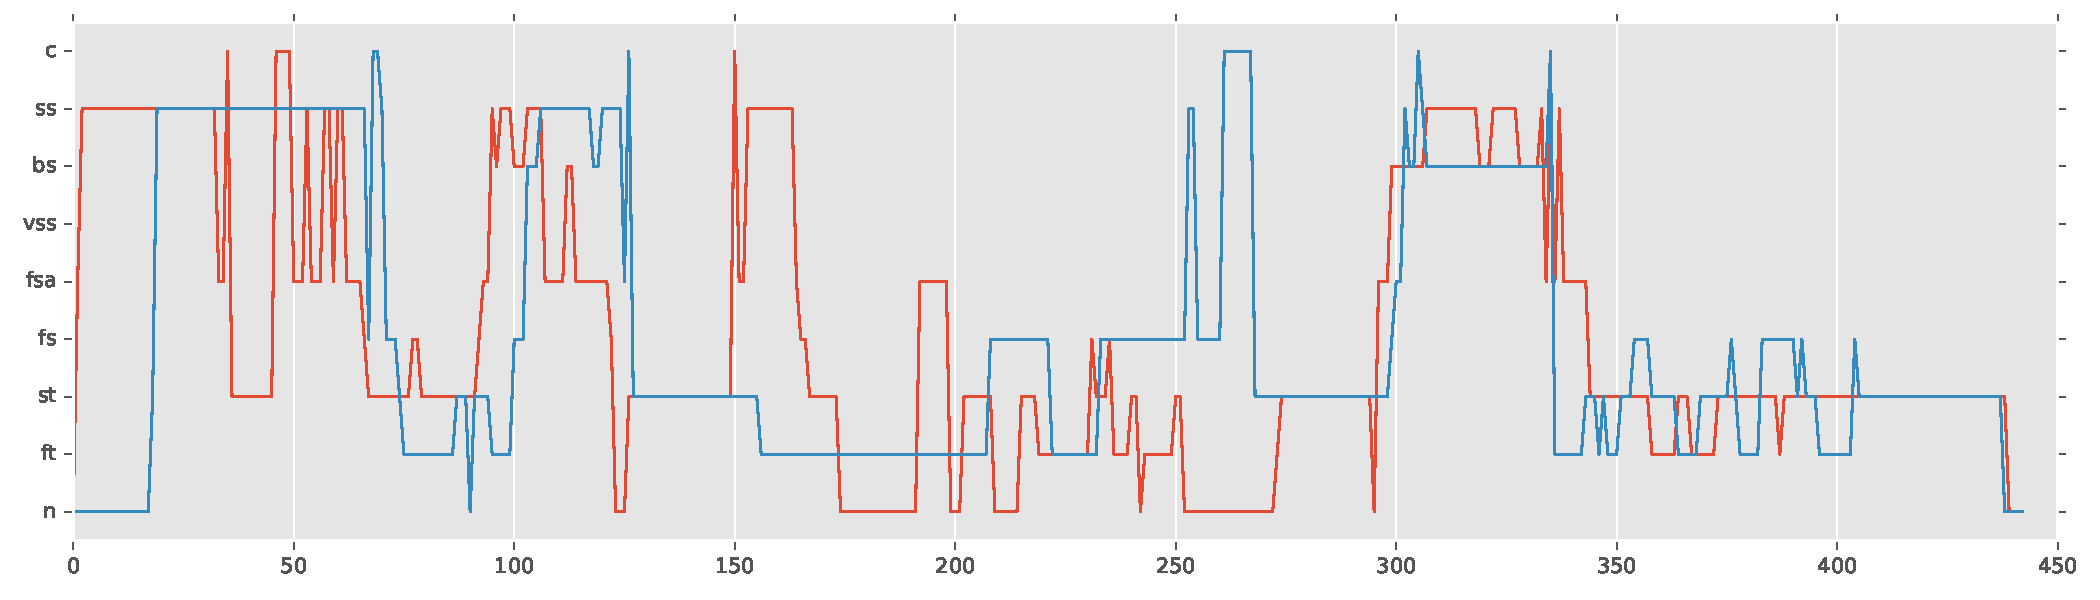
\includegraphics[width=\columnwidth]{duet-performance-512n-30ep-14}
  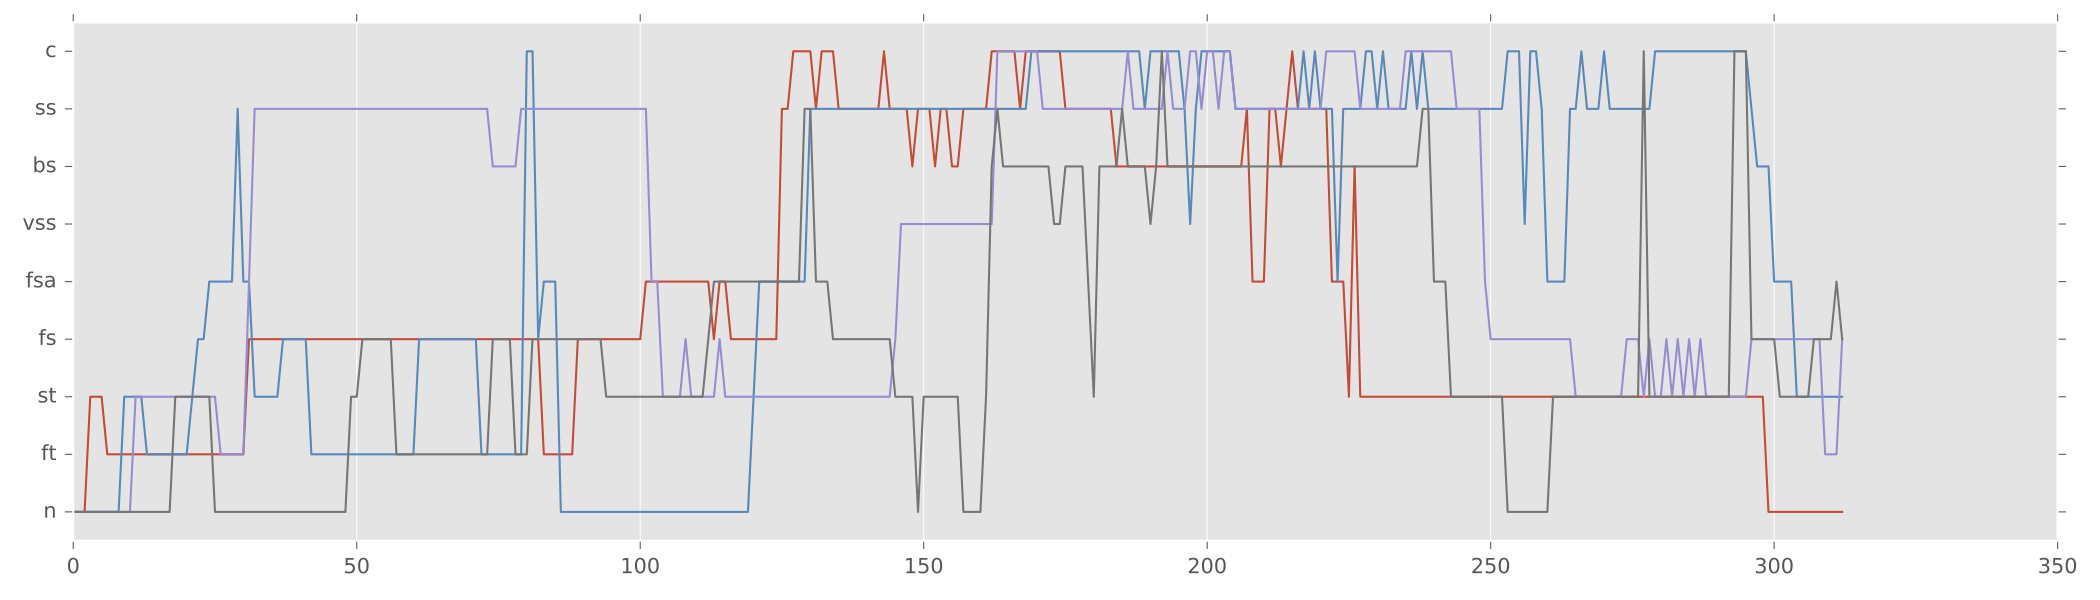
\includegraphics[width=\columnwidth]{quartet-performance-512nodes-16}
  \caption{A generated duet (above) and quartet (below) where one lead
    performer (shown in red) has been accompanied by ANN-generated
    performers. These results
    show some realistic ensemble interaction.}\label{fig:model-examples}
\end{figure}

The simplest ensemble configuration is a duet between two performers.
In this model, the input for the network is the current gesture of the
lead performer and the previous gesture of the second player while the
output is the current gesture of the second player. Training data was
constructed by taking each performer as leader and constructing
examples for each other player present in the performance. All
ensemble performances from the corpus were treated in this manner and
each sequence of 120 states was taken as a separate training example
resulting in a total of 319948 examples. The network was trained for
30 epochs taking 8.13 hours.

The upper part of Figure \ref{fig:model-examples} shows an example
output from the network with a lead player taken from a real
performance shown in red and a generated duo partner shown in blue.
The generated player's sequence was primed with the ``nothing''
gesture in the first state. The generated player shows a similar
complexity to the lead player and appears to mimic the leader's
gestures at some points.

\subsection{Quartet}

Performances with four players were the most numerous 
configuration in the corpus. In this model the input for the network
was the current gesture of lead player and previous gesture of the
three other players. The output was the predicted gestures for the
three others in the group.

Training data was constructed similarly to the duet model, with each
performer in the group considered as a lead player. As the ordering of
the other three players was significant in the encoding (but not in
the actual performance), a separate training example was constructed
for each permutation of players. The quartet model gesture-RNN was
trained on the whole data-set of 33 quartet performances with total
length of 5.28 hours corresponding to 19023 gesture state
measurements. The ANN was trained for 30 epochs on a corpus of 361560
examples; training time was 9.42 hours.

An example of a generated ensemble performance is shown in the lower
part of Figure \ref{fig:model-examples}. In this figure, the red line
shows a real gesture state sequence taken from a non-quartet
improvisation (not used to train the ANN), and the other three lines
show generated state sequences primed with the ``nothing'' gesture.

\section{Live Performance System}

The quartet gesture-RNN model was integrated into a live performance
system that sonifies the ensemble. This system allows a live performer
to interact with the the RNN's outputs as if it was a live group.
The system was created using an iPad app,
PhaseRings~\cite{Martin:2016ah}, and an ensemble director agent,
Metatone Classifier~\cite{Martin:2016xu}, that have been explored in
previous research but extended here to incorporate the gesture-RNN's
quartet model and synthesise audio outputs for the gesture sequences
produced by the generated ensemble parts.

The present system is illustrated in Figure
\ref{fig:live-performance-system}. One performer improvises with the
PhaseRings app. The performer's gestures are classified once every
second by Metatone Classifier. This gesture is used as the lead
performer input for the gesture-RNN. The ensemble inputs for this RNN
are initialised to the nothing gesture at the beginning of the
performance. Output gestures from the RNN are sonified in the
PhaseRings app running on three other iPads. An extension to Metatone
Classifier generates sequences of touch events that are sent to the
ensemble iPads in response to each signal from the gesture-RNN. These
touch sequences are produced concatenatively from 5-second chunks of
touch-data recordings from live performances with PhaseRings and other
iPad apps. The chunks have been labelled with their classified gesture
and a random chunk is chosen and streamed to each ensemble iPad every
five seconds or whenever a different gestural state is received from
the RNN.

\begin{figure}
  \centering
  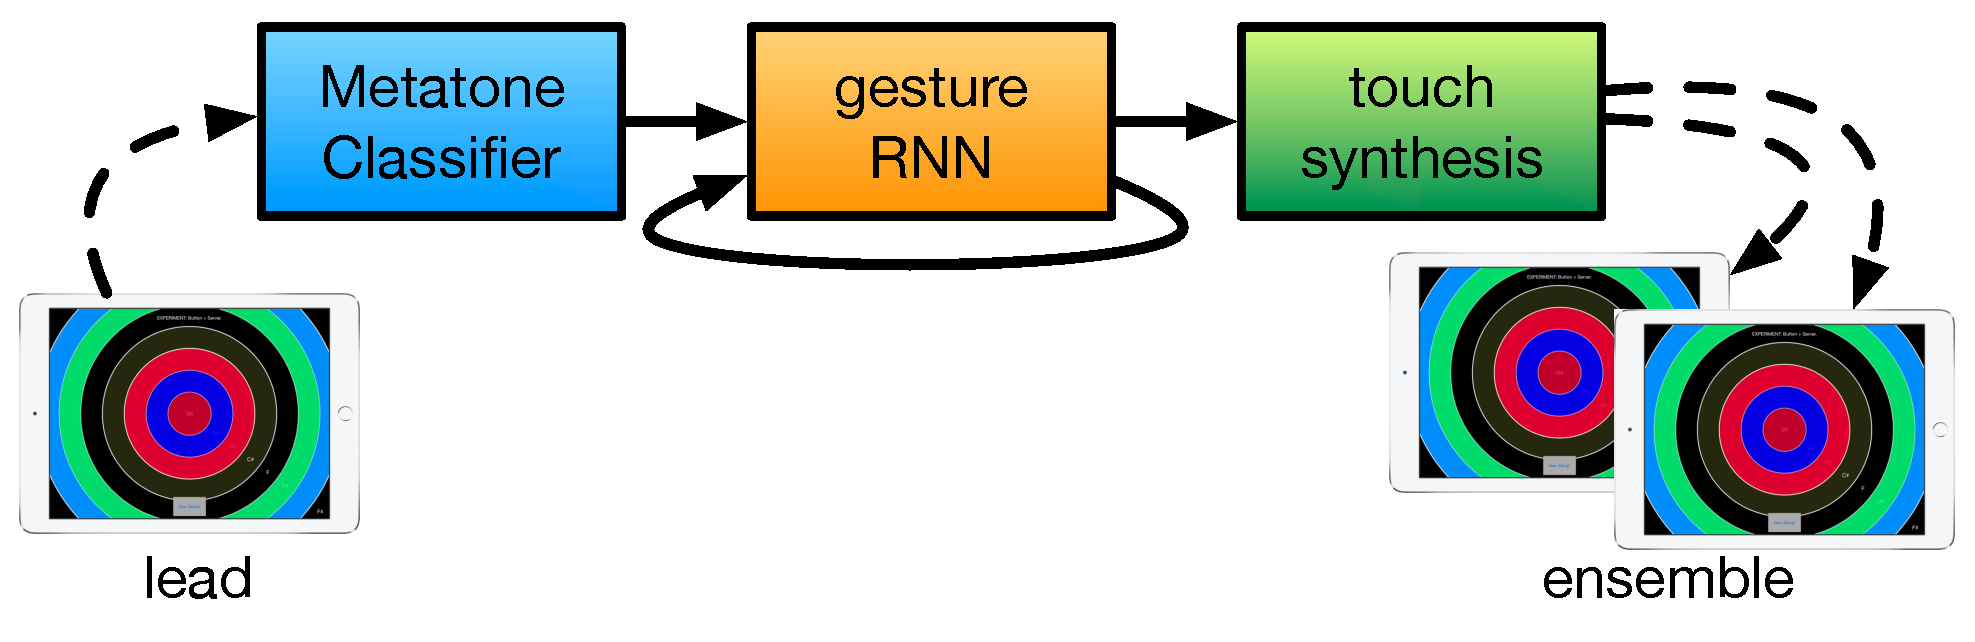
\includegraphics[width=\columnwidth]{live-performance-system}
  \caption{The live performance system classifies gestures from a live
  performer, generates ensemble gestures, then plays back synthesised
  touch events.}\label{fig:live-performance-system}
\end{figure}

\begin{figure}
  \centering
  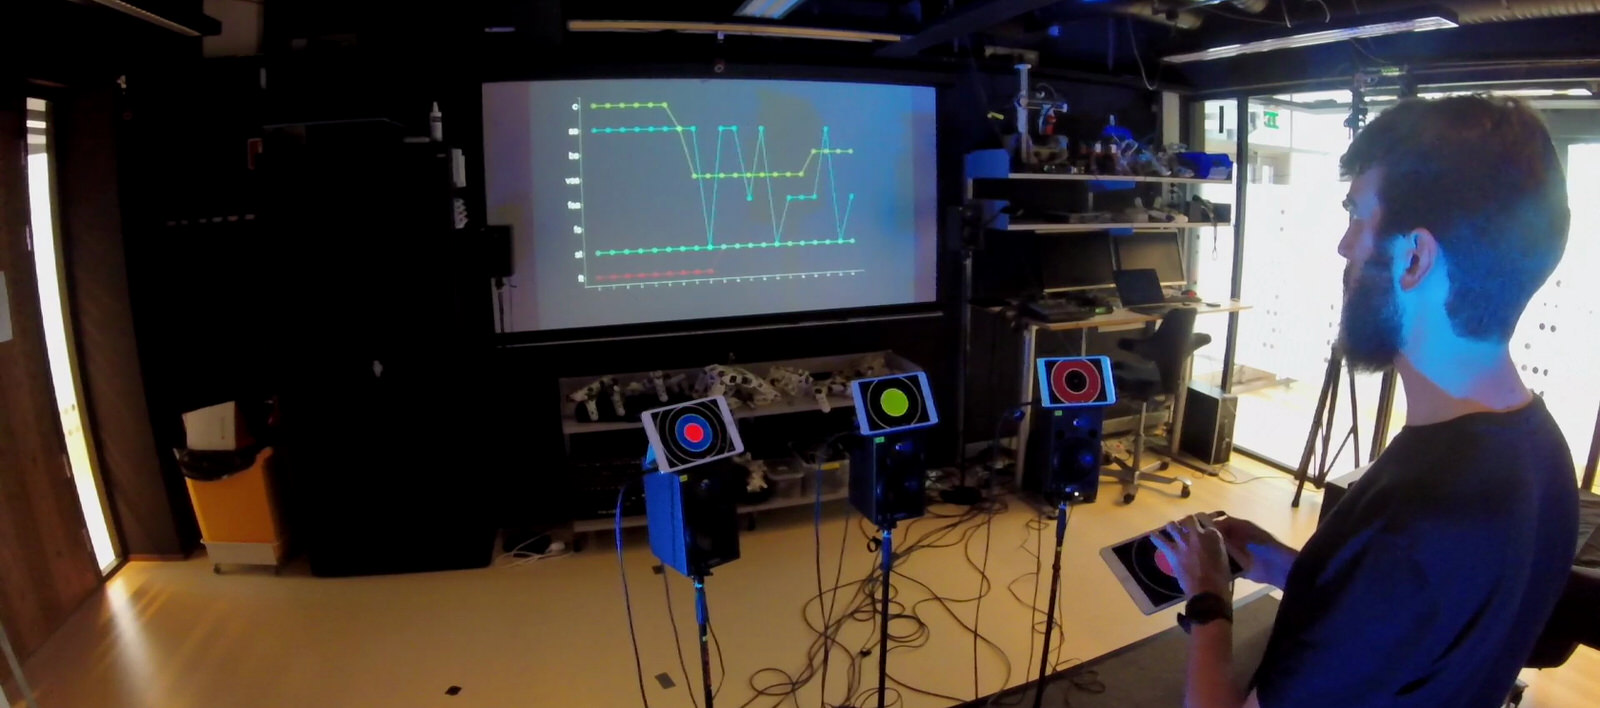
\includegraphics[width=\columnwidth]{neural-ipad-band-demo.jpg}
  \caption{A performance with the live performance system, a video is
    available at
    \url{https://doi.org/10.5281/zenodo.831910}}\label{fig:live-system-demo}
\end{figure}

So far, this live performance system has only been used within our
lab. The lead iPad rests on top of a monitor speaker where it can be
easily operated and heard by the performer. The two ensemble iPads are
connected to separate monitor speakers such that the performer can
hear them clearly as well as see the screens where the synthesised
touches are visualised. This setup is shown in the right side of
Figure \ref{fig:performance-and-system}. While PhaseRings was not
originally designed to playback touch interactions, the present system
is based on real performance data so the output from each iPad sounds
convincingly human. The app and agent system ensures that sounds
created in the ensemble are harmonically related, but since the timing
of notes between iPads are not connected, performances with the
system tend towards free rhythm. We envision that the present system
could be used in performances or installations that explore this
neural model of ensemble interaction. In this setup the separate
iPads and speakers embody the simulated ensemble and allow the
gesture-RNN's contribution to the performance to be examined. Other
performance situations, such as representing the ensemble performers
within a single app, may also be possible, and might allow individual
performers to enjoy ensemble-like experiences.

\section{Conclusions and Future Work}

This paper reports on work-in-progress towards a practical ANN model
of ensemble interaction for touch-screen performances. Unlike other
musical performance ANNs, the gesture-RNN creates transcriptions of
high-level gestures rather than individual notes and generates an
ensemble response to the gestures of a given lead performer.
Visualising the results suggests that realistic ensemble interactions
are being generated; however, further work needs to be done to show
that the generated ensemble responses are accurate and demonstrate
more interesting interactions than unrelated sequences. A live
performance system has been created that allows the gesture-RNN to
generate responses to a live performer and then sonifies the results
in real-time. This system could be used in live-performances,
installations, as well as to help evaluate the performance of the
gesture-RNN model.

\subsubsection*{Acknowledgements}
This work is supported by The Research Council of Norway as
a part of the Engineering Predictability with Embodied Cognition
(EPEC) project, under grant agreement 240862.

%\bibliographystyle{SIGCHI-Reference-Format}
\bibliographystyle{ACM-Reference-Format}
\bibliography{2013ComputerMusic}

\end{document}
